
%%%%%%%%%%%%%%%%%%%%%%%%%%%%%%%%%%%%%%%%%%%%%%%%%%%%%%%%%%%%%
%% Based on a TeXnicCenter-Template, which was             %%
%% created by Christoph Börensen                           %%
%% and slightly modified by Tino Weinkauf.                 %%
%%                                                         %%
%% Then, a third guy - me - put in some modifications.     %%
%%                                                         %%
%%                IFT3150 - Rapport                        %%
%%%%%%%%%%%%%%%%%%%%%%%%%%%%%%%%%%%%%%%%%%%%%%%%%%%%%%%%%%%%%

\documentclass[letterpaper,12pt]{scrartcl}
% Optimised for letter. Add ",twosides" to use the two-sides layout.

% Margins
    \usepackage{vmargin}
    \setpapersize{USletter}
    \setmargins{2.0cm}%	 % Left edge
               {1.5cm}%  % Top edge
               {17.7cm}% % Text width
               {21.0cm}% % Text height
               {14pt}%	 % Header height
               {1cm}%    % Header distance
               {0pt}%	 % Footer height
               {2cm}%    % Footer distance
				
% Graphical bugfix (about footnotes)
    \usepackage[bottom]{footmisc}

% Fonts and locale
	\usepackage{t1enc}
	\usepackage[utf8]{inputenc}
	\usepackage{times}
	\usepackage[francais]{babel}

	\AtBeginDocument {%
	    \renewcommand\tablename{\textsc{Tableau}}
	}

% Graphics
	\usepackage[pdftex]{graphicx}
	\usepackage{color}
	\usepackage{eso-pic}
	\usepackage{everyshi}
	\usepackage{float}
	\renewcommand{\floatpagefraction}{0.7}

% Enable hyperlinks
	\usepackage[pdfborder=000,pdftex=true]{hyperref}
	
% Table layout
	\usepackage{booktabs}

% Caption
	\usepackage{ccaption}
	\captionnamefont{\bf\footnotesize\sffamily}
	\captiontitlefont{\footnotesize\sffamily}
	\setlength{\abovecaptionskip}{0mm}

% Header and footer settings
	\usepackage{scrpage2} 
	\renewcommand{\headfont}{\footnotesize\sffamily}
	\renewcommand{\pnumfont}{\footnotesize\sffamily}

% Pagestyles
	\defpagestyle{cb}{
		(\textwidth,0pt) % Sets the border line above the header
		{\pagemark\hfill\headmark\hfill} % Doublesided, left page
		{\hfill\headmark\hfill\pagemark} % Doublesided, right page
		{\hfill\headmark\hfill\pagemark} % Onesided
		(\textwidth,1pt)} % Sets the border line below the header
		{(\textwidth,1pt) % Sets the border line above the footer
		{{\it Plan MUS2323}\hfill François Poitras} % Doublesided, left page
		{François Poitras\hfill{\it Plan MUS2323}} % Doublesided, right page
		{François Poitras\hfill{\it Plan MUS2323}} % One sided printing
		(\textwidth,0pt) % Sets the border line below the footer
	}

% Footnotes
	\renewcommand{\footnoterule}{\rule{5cm}{0.2mm} \vspace{0.3cm}}
	\deffootnote[1em]{1em}{1em}{\textsuperscript{\normalfont\thefootnotemark}}

% Document specific
\usepackage{hyperref}
\usepackage{amssymb}
\pagestyle{empty}

\begin{document}
	\begin{center}
		\vspace{2cm}

		{\Huge\bf\sf Rapport de projet}
		\vspace{4cm}

		{\bf\sf Par}

		\vspace{0.5cm}{\large\bf\sf François Poitras}

		\vspace{2cm}

		{\bf\sf Présenté à}

		\vspace{0.5cm}{\large\bf\sf Olivier Bélanger et Sylvie Hamel}

		\vspace{2cm}

		{\bf\sf Dans le cadre du cours de}

		\vspace{0.5cm}{\large\bf\sf Projet d'informatique (IFT3150)}

		\vspace{\fill}
		
		\today

		\vspace{0.5cm}
		Université de Montréal
	\end{center}

	\newpage
	\tableofcontents
	\newpage
	\pagestyle{plain}
	\section{Plan de travail initial}
	
	\subsection{Énoncé}
	Il s'agit de complémenter une application qui permet actuellement à l'utilisateur de construire des progressions d'accords arbitraires. Le but du projet est de permettre au programme de construire une mélodie agréable qui accompagne les accords. Pour ce faire, il faut tout d'abord déterminer quelle est la tonalité de la progression. Ensuite, il faut établir quelle(s) gammes peuvent être utilisées, en se basant sur les notes des accords présents. Vient ensuite la partie la plus difficile, celle où il faut développer des idées musicales de manière pseudo-réaliste et non simplement jouer des notes de la gamme au hasard. Bien sur, il y aura une partie de hasard dans le choix des notes ou des phrases, mais l'idée est d'implémenter des structures qui permettent de générer une mélodie «écoutable». Pour ce faire, différentes avenues seront explorées, en se basant sur les lectures préliminaires. La base du moteur audio est pyo \cite{pyo}.

Pour ce qui est de la basse, la technique devrait d'être plus simple. On peut simplement implémenter quelques recettes et les varier au fil des mesures. Par exemple, on peut jouer la fondamentale sur le temps 1, jouer une note de l'accord sur le temps 2 et jouer une note différente sur le temps 3. Pour le quatrième temps, on approche l'accord suivant, par exemple avec du chromatisme. 

Si le temps le permet, des synthétiseurs additionels seront développés pour varier l'instrumentalisation du programme, autant pour les accords que pour la mélodie ou la basse. Pour aider au développement d'éventuels synthétiseurs, la lecture de la série "Synth Secrets" de la revue Sound on Sound pourra aider. Ce développement se fera en parallèle des étapes mentionnées dans l'échéancier, il ne consiste pas en une étape en tant que tel. 

Note : L'application a déjà été commencée dans le cadre du cours MUS3327 à l'Hiver 2017. La partie sur les progressions d'accord a été développée dans ce cours. Au moment de débuter le projet, l'application génère également une ligne de basse plutôt primitive. Aucun calcul n'est fait sur celle-ci, elle ne fait que suivre les accords. Tout le code est disponible à l'adresse suivante : 

\href{https://github.com/poifra/Creamuspython2}{https://github.com/poifra/Creamuspython2}. Il s'agit du dépôt utilisé pour le cours MUS3327 avec les fonctionalités supplémentaires développées dans le cadre du projet.

	\subsection{Résumé du développement}
	\subsubsection{Échéancier}
	\begin{itemize}
	\item 7 mai	\\
	J'ai commencé la recherche d'articles pour avoir une idée de l'approche à utiliser. Plusieurs articles utilisent des processusus stochastiques comme des chaînes de Markov pour construire des séquences de notes intéressantes. Une autre approche consiste à considérer les règles d'harmonies musicale comme une grammaire d'une langue naturelle. Ainsi, on peut appliquer des techniques de traitement de langue à des «phrases» musicales, tout en gardant nécéssairement une composante aléatoire. Ce sont les deux méthodes qui semblent le plus prometteuses. Une troisième approche serait d'utiliser des techniques d'apprentissage machine pour générer des mélodies, mais considérant le temps disponible pour réaliser le projet, cette approche ne sera pas explorée. En effet, le temps d'apprentissage semble plutôt long et l'implémentation demanderait aussi trop de temps. 

Les deux méthodes mentionnées semblent toutefois avoir l'inconvénient de se baser sur du matériel existant pour établir les transitions enre les notes. Des recherches plus approfondies seront nécéssaires pour déterminer dans quel mesure il est possible de créer une improvisation à partir uniquement d'une séquence d'accords 

	\item 20 mai \\
	En raison d'un problème de santé, la rencontre prévue avec Olivier n'a pas pu avoir lieu et donc le travail n'a pas pu débuter aussi rapidement que prévu. Nous essayons présentement de trouver une autre date. J'ai également décidé de ne pas développer d'algorithme permettant la reconnaissance d'une tonalité, à partir d'une séquence d'accords. Bien qu'il soit théoriquement possible de le faire, il existe trop d'ambiguités qu'un programme de peut pas résoudre. En effet, un musicien pourrait décider d'utiliser une séquence d'accords qui n'harmonise aucune gamme, par exemple : G - B - C - Cm. Cette progression est utilisée dans la chanson \textit{Creep} de Radiohead. On remarquera qu'il y a un Do majeur et un Do mineur, ce qui rend une analyse simple impossible. Je vais plutôt ajouter une boîte de texte dans l'application qui demande à l'utilisateur quelle tonalité utiliser. De cette façon, même si il y a des "accidents", le programme aura une idée de quelle tonalité utiliser. La programmation d'une ligne de basse mélodique risque de prendre un peu de retard, mais elle devrait commencer sous peu. L'horaire du projet a aussi été revu, pour prendre en compte le fait que la présentation aura lieu plus tard que prévu initialement.
	\item 1er juin\\
	Après une rencontre avec Olivier, nous avons pu établir les grandes orientations du projet. Premièrement, le moteur sera développé de façon séparée de l'interface, afin qu'il soit éventuellement inclu dans pyo-tools. Olivier m'a également suggéré la lecture du livre que j'avais trouvé dans mes recherches initiales (voir premier rapport). 

Suite aux discussions, j'ai décidé d'utiliser une approche intrinsèquement aléatoire dans la génération de mélodie. L'autre méthode serait de rechercher des banques MIDI afin d'utiliser des chaînes de Markov. Olivier m'a suggéré d'étudier le fonctionnement des classes de pyo qui utilisent de l'aléatoire afin de m'en insipirer. 
J'ai également commencé à réfléchir à la structure que je veux utiliser pour la "walking bass". Celle-ci va utiliser des règles plutôt fixes qui vont faire en sorte que la mélodie de basse va bien fonctionner. Le programme ne devrait pas souvent gébérer deux fois la même ligne, mais celles-ci risquent de se ressembler.
	\item 14 juin\\
	La walking bass est fonctionnelle. Celle-ci est une version à peine plus complexe de la version d'origine. La basse joue uniquement des noires, donc quatre notes par mesure. Le premier temps est la tonique, c'est-à-dire la note fondamentale de l'accord courant. Le deuxième temps est une note aléatoire de la gamme (mineure ou majeure, selon le cas) correspondante. Le troisième temps est une des notes composant l'accord (par exemple la tierce, la quinte ou la septième) choisie aléatoirement. Finalement, le dernier temps est une note d'approche, c'est à dire une note qui est un demi-ton sous la tonique de l'accord suivant. Des améliorations sont possibles. Par exemple, l'algorithme pourrait s'assurer de ne pas jouer deux fois la même note de façon consécutive, pour que la mélodie de basse soit plus intéressante. Aussi, lors de tests, j'ai remarqué que la gestion du tempo n'était pas bien implémentée et devra être corrigée dans la version finale. 
	\item 28 juin\\
	J'ai implémenté différents générateurs aléatoires. Ils sont basés sur les générateurs présents dans pyo. La prochaine étape consiste à tester les différentes distributions (uniforme, gaussienne, Poisson, etc.) implémentées pour voir si certaines produisent des résultats plus intéressants. Je ne suis pas certain de la méthode que je veux adopter pour relier les générateurs à des notes MIDI, mais la librairie possède une fonction snap qui a un comportement similaire. Il est possible que je m'en inspire. Actuellement, tous les générateurs donnent un flottant compris dans l'intervale [0, 1[. En raison des retards dans l'horaire prévu, il est possible que la programmation de mélodies aléatoires ne soit pas terminée selon l'échéancier initial.
	\item 10 juillet\\
	J'éprouve quelques difficultés à contacter Olivier pour lui poser des questions sur l'orientation du projet. Entre autres, l'implémentation que j'ai utilisée pour les générateurs semble extrêmement biaisée. Pour l'instant, je teste les différents générateurs avec une fonction snap qui fait en sorte de relier une distribution de valeurs à une gamme quelquoncque. Toutefois, les résultats ne sont pas très intéressants au niveau musical. Il pourrait être intéressant de développer des générateurs plus complexes, qui font appel à des motifs musicaux générés précédemment. Il y a aussi l'aspect rythmique de la mélodie qui n'a pas encore été travaillé. Il pourrait être possible d'implémenter les motifs rythmiques les plus communs et de tenter de les combiner à la génération aléatoire.
	\item 24 juillet\\
	Je suis présentement en train de relier les générateurs aléatoires au moteur audio développé plus tôt au cours du projet. L'idée est la même que pour la walking bass, c'est à dire que l'accord courant est utilisé comme base. Un ensemble de notes est généré, basé sur une distribution aléatoire. Il va bientôt être possible (d'ici environ une semaine) de juger de la qualité de l'improvisation ainsi générée. Cependant, je pense qu'il va falloir appliquer d'autres techniques pour avoir un résultat décent. Par exemple, il pourrait être possible de ré-utiliser certains passages générés précédemment et de les varier un peu. On peut aussi biaiser un générateur aléatoire afin qu'il produise plus de notes qui harmonisent l'accord courant, plutôt que simplement des notes d'une gamme.

	\item 19 août\\
	Envoi du rapport.
	
	\end{itemize}

	\section{Résultats}
	La ligne de basse est correcte. Elle est fixée à un tempo qui est le double de celui des accords. Comme les accords sont des blanches, le tempo est donné par la basse et agit comme un métronome. Ceci a été fait afin de simplifier le processus de synthèse. En donnant la gestion du tempo à la basse, il est ainsi possible d'éviter la synthèse d'une batterie, qui aurait nécéssité du temps sans rien apporter aux résultats mélodiques. Toutefois, il est évidemment possible d'améliorer la basse, mais elle joue son rôle efficacement dans l'implémentation actuelle. Pour plus de détails concernant les améliorations mélodiques, voir la section sur les perspectives. 
	
	La méthode utilisée, qui consiste à se baser uniquement sur des données pseudo aléatoire, n'est pas très efficace. Il s'agit d'une bonne base, mais cette méthode doit être couplée à d'autres méthodes, qui n'ont pas été explorées dans ce projet, pour donner de meilleurs résultats. Les rèlges harmoniques implémentées ne sont pas suffisantes. 

	\subsection{Générateurs aléatoires}
	L'élément qui a été plus complexe à modéliser est la mélodie proprement dite. En effet, créer une mélodie qui respecte une tonalité est plutôt simple en soi. La base de la génération est basée sur différentes distributions aléatoires, qui, pour faciliter leur traitement subséquent, sont $\mathbb{R} \in [0,1]$. Tous les générateurs sont définis dans la classe \textit{MyRandoms}. La distribution la plus simple est uniforme et sert de base pour les autres. Évidemment, cette distribution est pseudo-aléatoire, mais la distinction est négligeable dans ce projet, puisqu'il n'y a pas de contraintes de sécurité. L'ensemble des générateurs utilisent soit 0, 1 ou 2 paramètres pour fonctionner \cite{args1} \cite{args2}. La classe qui gère les générateurs a été codée de façon a permettre l'ajout de nouvelles fonctions du même format. 
	
	Une fonction de \textit{map} a été créer afin de relier un ensemble de valeur réelles à des notes MIDI. Étant donné une gamme de $n$ notes et une distribution $d$ aléatoire, la fonction calcule l'écart $r$ de la fonction, c'est à dire $max(d) + |min(d)|$ et crée $\frac{r}{n}$ index. Ensuite, la fonction attribue à chaque valeur de $d$ un index qui sera forcément compris entre 0 et $n$ et recherche cet index dans le tableau qui représente la gamme.
	
	Le problème le plus important de la mélodie générée dans la version actuelle est l'absence de «phrases» musicales. En effet, dans la très grande majorité des solos en musique, on peut décortiquer les différentes parties en phrases, un peu comme dans une langue naturelle. On peut par exemple avoir des pauses, mettre l'accent sur une certaine idée, etc. Dans la version actuelle, le générateur de mélodie ne possède pas la capacité de construire des phrases bien définies et on pourrait qualifier le résultat de monotonne. Comme un discours monotonne, il est donc difficile de déterminer quelle idée le message tente d'envoyer.
	
	\subsubsection{Générateurs particuliers}
	Deux générateurs ne se qualifient pas tout à fait d'aléatoires. Il s'agit des modes \textit{walker} et \textit{loopseg}. Le premier commence par une valeur arbitraire et l'algorithme tire à pile ou face pour déterminer le mouvement de la séquence. Dans la moitié des cas, la valeur de la séquence augmente d'une petite valeur et dans l'autre cas, elle diminue d'une petite valeur. Cette valeur est déterminée par le paramètre $x_2$ de la fonction. Plus le paramètre est grand, plus la valeur peut varier. Le paramètre $x_1$ contrôle la valeur maximale que peut retourner la fonction.
	
	L'algorithme du \textit{loopseg} utilise la même méthode, mais avec une étape supplémentaire. Un buffer est gardé en mémoire pour stocker les valeurs précédemment générées. Cela fait en sorte qu'après avoir généré \textit{loopLen} valeurs, l'algorithme change de mode pour utiliser  les valeurs créées précédemment. Donc, au lieu de générer de nouvelles valeurs, l'algorithme va utiliser des valeurs existantes. Cela imite une technique d'improvisation classique qui consiste à reprendre des idées ou des concepts musicaux déjà utilisés plus tôt dans un solo. Il s'agit de l'algorithme qui semble donner les meilleurs résultats et il aurait été possible, avec plus de temps, d'inclure plus d'idées en ce basant sur le \textit{loopseg}.
	
	\subsection{Problèmes rencontrés}
	L'appréciation de l'improvisation est évidemment subjective, en autant que la mélodie soit dans la même tonalité que la progression d'accord. Cette règle n'est toutefois pas absolue, mais pour simplifier la mélodie, nous assumerons qu'elle est nécéssaire. Le résultat est donc correct, sans être extraordinaire. La mélodie respecte la tonalité, mais son principal point faible est l'absence de structures rythmiques claires. Chaque note a une durée qui est respectée par rapport au tempo, mais l'ensemble de la mélodie de présente pas forcément de cohérence rythmique. Il s'agit de l'aspect qui, étonamment, a été le plus difficile à modéliser. Le choix de notes n'est pas trop complexe, mais donner une saveur rythmique à la mélodie a été un défi plus important que prévu. 
	
	En raison du temps mis à développer les générateurs et en raison de la difficulté à communiquer avec Olivier au cours de l'été, le rythme de travail a été beaucoup moins important que prévu. Il a fallu dans un premier temps adapter le programme développé dans le cours de MUS3327 pour qu'il supporte un moteur indépendant. La gestion globale du temps pour la basse et les accords a posé un défi dans une moindre mesure, car les deux sont intrinsèquement liés. Afin de faciliter le rendu final, la gestion du temps de la mélodie n'est pas reliée au temps global. Cela fait qu'il est difficile de synchroniser les notes individuelles de la mélodie avec les accords, ce qui réduit l'efficacité de la composition. On pourrait par exemple vouloir faire en sorte, comme avec la basse, que la mélodie joue une tonique de l'accord sur un temps fort, ou encore qu'elle commence par un arpège rapide de l'accord. 
	
	La principale difficulté vient du fait que le compteur global de temps compte des noires (ou des blanches, dans le cas des accords). Or, dans la plupart des oeuvres musicales, rien n'oblige le musicien à jouer sur les temps fixes. Un musicien va généralement chercher à commencer ou terminer une phrase sur un temps précis, mais pour ce qui se passe entre le début et la fin, presque tous les coups sont permis. D'un point de vue algorithmique, cette idée est difficile à représenter. Supposon que l'on veille construire une phrase de 8 temps. Il est facile de décider à quel endroit commencer. Ensuite, nous produisons aléatoirement un ensemble de notes qui on une durée qui varie entre une noire et une double croche. Comme nous ne connaissons pas d'avance la durée des notes générées, il est difficilement possible de savoir quelle doit être la durée de la dernière note pour terminer la phrase sur un temps précis. Dans l'exemple si-dessous, on remarque à plusieurs endroits des notes qui « débordent » dans la mesure suivante, comme entre les mesure 2 et 3, ainsi que les mesures 4 et 5.
	
\begin{figure}[H]
\caption{Exemple de quelques phrases sur huit mesures (extrait du solo de guitare de \textit{Sunshine Of Your Love})}
\centering
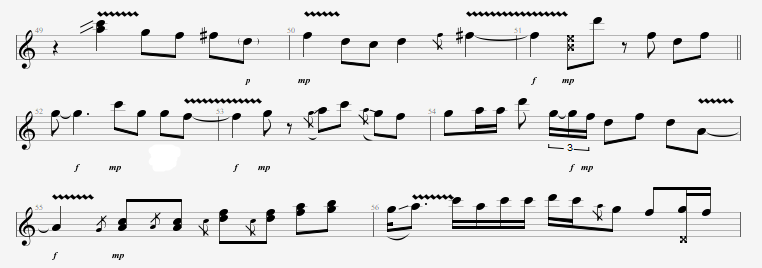
\includegraphics[scale=0.5]{phrase.png}
\end{figure}	
	
	\section{Perspectives}
	
	Ce genre de projet est de ceux qui peuvent être développés pendant extrêmement longtemps. Toutefois, si le développement de ce compositeur automatique continue, certaines avenues doivent être priorisées. Cette section décrit les principales possibilités, que ce soit au niveau du moteur mélodique ou encore de l'interface utilisateur.
	
		\subsection{Mélodie}
		Dans la version actuelle, la plupart des paramètres qui contrôlent la génération musicale sont \textit{hardcodés} dans le code, comme par exemple l'algorithme utilisé pour la mélodie, les paramètres des fonctions aléatoires, etc. Il pourrait être intéressant d'ouvrir ces paramètres à l'utilisateur pour lui permettre de personnaliser le résultat selon ses goûts. De plus, cela pourrait permettre d'explorer plus facilement les différentes facettes des algorithmes implémentés. Un contrôle sur le volume des différents synthétiseurs serait aussi souhaitable, afin de faciliter la recherche d'un équilibre sonore.
		
		Tel qu'il a été discuté dans les sections précédentes, la mélodie est relativement simpliste et pourrait bénéficier de techniques plus avancées, en ce qui concerne le choix de notes et de rythmes. En particulier, si l'on garde une base aléatoire. Le livre de Gerard Nierhaus\cite{nierhaus}, mentionné dans le rappel de l'échéancier, mentionne entre autres des techniques d'algorithmes génétiques, de grammaires génératives, de modèles Markoviens et d'automates cellulaires. Le problème est l'approche généraliste de Nierhaus, qui fait en sorte qu'il peut être difficile de se baser uniquement sur son ouvrage pour implémenter différentes approches.
		
		Si l'on abandone l'idée de se baser uniquement sur des données aléatoires, il devient alors possible d'inclure des notions d'apprentissage machine dans l'objectif de répliquer des styles de musiciens connus. Par exemple, on peut penser qu'avec une base de données suffisament grande de répertoire jazz, il serait possible pour un algorithme d'apprentissage de remarquer et d'utiliser des motifs présents dans cette hypothétique base de données.
		\subsection{Basse et accords}
		La principale améloriation pour ce qui est de la ligne de basse est surtout rythmique. En effet, on peut imaginer qu'au lieu de jouer simplement des noires, on veille calquer la basse sur les accords, c'est-à-dire sur des blanches ou encore des rondes. L'autre améloriation possible est de transformer les accords et la basse en triolets afin de créer un rythme \textit{swing}, typique du jazz et du blues. Bien sur, si on adopte une base rythmique différente, il peut être souhaitable que la mélodie suive, bien que des mélanges peuvent co-exister.

\begin{figure}[H]
\centering
\caption{Exemple de \textit{swing feel} \cite{swing} }
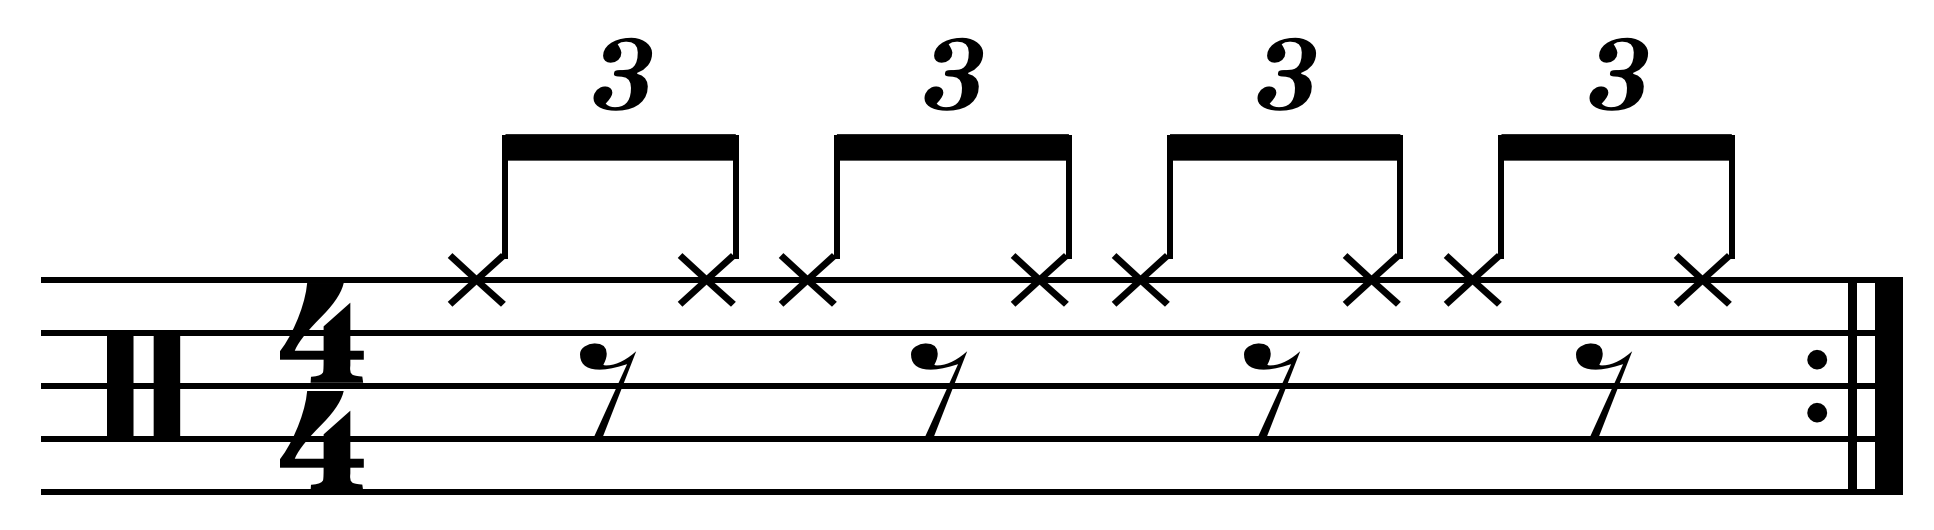
\includegraphics[scale=0.1]{shuffle.png}
\end{figure}	

	Spécifiquement sur la question des accords, il pourrait être intéressant de permettre à l'usager de modifier leur \textit{voicing}, c'est à dire la façon dont l'accord de présente. Par exemple, un Do majeur s'écrit normalement (du plus grave au plus aigu) Do - Mi - Sol, mais il est possible de renverser le Mi --- et le sol --- pour obtenir par exemple, Mi - Sol - Do. Dans la version initiale du cours MUS3327, les inversions de n'importe quelle basse étaient prévues, on pouvait donc avoir un Do majeur avec une basse de Si bémol. Toutefois, pour des raisons de simplicités, seules les inversions de toniques sont en partie présentes dans la version finale. 
		
	\subsection{Style musical}
		L'idée initiale était de développer un moteur simulant des instrumentalisations de jazz. Bien que le résultat final soit plutôt éloigné de ce style, il est possible d'envisager qu'en combinant les variations mentionées dans les sections précédentes, on arrive à créer des styles différents. En généralisant grossièrement, on peut par exemple supposer qu'un utilisateur entre une progression de \textit{power chords} (comprenant uniquement la fondamentale et la quinte) avec un rythme soutenu de croches. Cela donnerait alors un style beaucoup plus rock, voir métal, à la musique produite. 
		
	Une autre améloriation en ce sens serait de laisser à l'usager la possibilité de choisir plus qu'un accord par mesure et de permettre d'autres métriques que $\frac{4}{4}$. Dans un premier temps, l'utilisateur pourrait avoir le choix entre d'autres métriques communes, comme $\frac{3}{4}$ ou $\frac{12}{8}$ pour aller progressivement vers une version où l'usager est complètement libre.

		\subsection{Éléments graphiques}
		L'interface graphique en tant que tel est assez intuitive à utiliser, mais la construction elle même de progression d'accords pourrait être révisée. Dans la version actuelle, les accords sont représentés par une pile. Pour remplacer le premier accord de la progression, il faut donc dépiler tous les accords avant de pouvoir modifier le premier.
		
		 La solution la plus simple serait de demander à l'usager à quelle position il veut placer l'accord qu'il a choisit. Par contre, il pourrait être difficile d'implémenter cette fonction sans alourdir considérablement l'interface. Une solution plus complexe est d'implémenter un système de \textit{drag and drop}, tel que mentionné dans le plan initial. De cette façon, l'utilisateur pourrait déplacer à sa guise les accords qu'il a placé et cela garderait l'esprit intuitif de l'interface.

\section{Bibliographie} 
\begin{thebibliography}{9}
   
   \bibitem{pyo} \href{http://ajaxsoundstudio.com/software/pyo/}{Pyo, dedicated Python module for digital signal processing}
   
   \bibitem{nierhaus}
          Gerhard Nierhaus,
          \emph{Algorithmic Composition : Paradigms of Automated Music Generation}.
          Springer-Verlag/Wien, Allemagne,
          273 p.
          2010.
          
    \bibitem{cluster} \href{http://wesscholar.wesleyan.edu/cgi/viewcontent.cgi?article=1344&context=etd_hon_theses}{A Clustering Algorithm for Recombinant Jazz Improvisations}, Jonathan Gillick, Wesleyan University, Connecticut
    
	\bibitem{techniques} \href{http://peterlangston.com/Papers/amc.pdf}{Six Techniques for Algorithmic Music Composition} \emph{Peter S. Langston}, Morristown, New Jersey

	\bibitem{model} \href{http://www.ece.umd.edu/~blj/algorithmic_composition/algorithmicmodel.html}{Algorithmic Composition as a Model of Creativity}, Bruce L. Jacob, University Of Michigan
	
	\bibitem{algo} \href{https://en.wikipedia.org/wiki/Algorithmic_composition}{Algorithmic Composition, Wikipedia}
	
	\bibitem{swing} \href{https://en.wikipedia.org/wiki/Swing_(jazz_performance_style)}{Swing (jazz performance style)}, Wikipedia
	
	\bibitem{phrase} \href{https://en.wikipedia.org/wiki/Phrase_(music_theory)}{Phrase (music theory)}, Wikipedia

	\bibitem{args1} \href{https://docs.python.org/2/tutorial/controlflow.html#arbitrary-argument-lists}{Python : Arbitrary argument Lists}
	
	\bibitem{args2} \href{https://stackoverflow.com/questions/1769403/understanding-kwargs-in-python}{Stackoverflow : Understanding kwargs in python}
\end{thebibliography}


\end{document}